\section{Template complex zonotopes}~\label{sec:tcz}
\paragraph{\bf Definition.}
A template complex zonotope is a set representation in which each point
is described as a linear combination of a set of complex-valued vectors,
called as a \textit{template}, such that the complex combining coefficients are
bounded in absolute values by a set of positive bounds called
\textit{scaling factors}.
%
\begin{defn}[Template complex zonotope]
  For $n,m\in\pint$, let $V\in\mCnm$ be a template, $c\in\mCn$
  be a center point and $s\in\mRmo$ be scaling factors.  Then we
  define a template complex zonotope as 
  \[\cz{V}{c}{s}=\lt\{V\zeta+c:\zeta\in\mCm~\wedge~\forall
  i\in\{1,\ldots,m\},|\zeta_i|\leq s_i\rt\}.\]
\end{defn}
%
Complex zonotopes, which were introduced in~\cite{arvind2016lis}, are
a special case of template complex zonotopes where $s_i = 1$ for all
$i\in\{1,...,m\}$.  The real projection of a template complex zonotope
can represent, in addition to polytopic zonotopes, non-polyheral
convex sets.  Therefore, they are also more expressive than usual
(real-valued) zonotopes.  To illustrate, Figure~\ref{fig:cz}
represents the non-polyhedral real projection of the template complex
zonotope $\CZO$ where $V=\lt(\begin{array}{lll}(1+2i) & 1 &
  (2+i)\\(1-2i) & 1 & (2-i)\end{array}\rt)$ and $s=[1~1~1]^T$.
%
\begin{figure}
\center
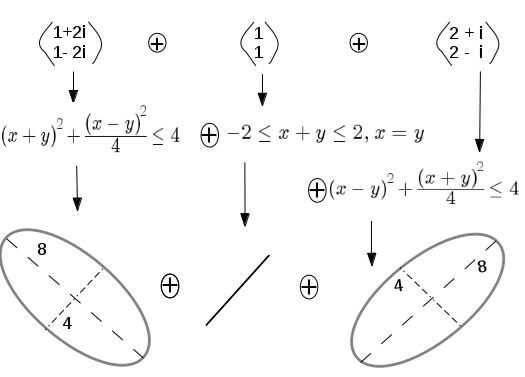
\includegraphics[scale=0.7]{fig/complex-zonotope.png}
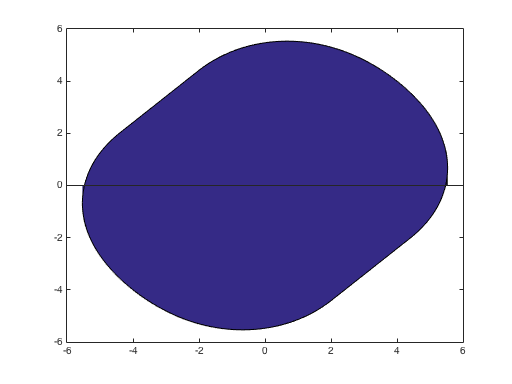
\includegraphics[scale=0.5]{fig/CZhull.png}
\caption{Real projection of a template complex zonotope}
\label{fig:cz}
\end{figure}
%




In the rest of the paper, unless otherwise stated, we assume that $V$
is an $n\times m$ complex matrix, $s$ is an $m\times 1$ column vector
and $c$ is a $n\times 1$ column vector for $m,n\in\pint$.

\paragraph*{\bf Operations on template complex zonotopes}
Concerning linear transformation and the Minkowski sum, computations
on template complex zonotopes are similar to those on usual (real-valued) zonotopes
as stated in the following results, which can be proved by the same
techniques as that of a usual zonotope. %~\cite{todo}.
%
\begin{lem}[Linear transformation and Minkowski sum]~\label{lem:lt}
  Let $A\in\mCnn$, $V\in\mCnm$, $G\in\mat{n}{r}{C}$, $c,d\in\mCn$, $s\in\mRmo$,
  $h\in\mb{R}^r_{\geq 0}$ for some $n,m,r\in\pint$.
  
\begin{enumerate}%\begin{equation}\label{eqn:lin} 
\item \emph{Linear transformation}: $A\CZ=\cz{AV}{Ac}{s}$.
\item \emph{Minkowski sum}: $\CZ\oplus\cz{G}{d}{h}=\cz{\lt[V~~G\rt]}{(c+d)}{\lt(\begin{array}{l}s\\h\end{array}\rt)}$.
%\end{equation}
\end{enumerate}
\end{lem}
%% \begin{proof}
%% $A\CZ=\{A(V\zeta +c):
%% |\zeta_i|\leq s_i~\forall i\in\tup{m}\}=\cz{AV}{Ac}{s}$.
%% \end{proof}
%
%% The Minkowski sum of two template complex zonotopes is another
%% template complex zonotope computed as follows.
%% %
%% \begin{lem}[Minkowski sum]\label{prop:op}
%%   Let $V\in\mCnm$, $G\in\mat{n}{r}{C}$, $c,d\in\mCn$, $s\in\mRmo$,
%%   $h\in\mb{R}^r_{\geq 0}$ for some $n,m,r\in\pint$.  Then
%% \begin{equation}\label{eqn:msum}
%% \CZ\oplus\cz{G}{d}{h}=\cz{\lt[V~~G\rt]}{(c+d)}{\lt(\begin{array}{l}s\\h\end{array}\rt)}
%% \end{equation}
%% \end{lem}
%% \begin{proof}
%% $\CZ\oplus\cz{G}{d}{h}\\=\{V\zeta+G\zeta^\pr+c+d:|\zeta_i|\leq s_i\forall
%% i\in\tup{m}~\wedge~|\zeta^\pr_j|\leq h_j\forall j\in\tup{r}\}\\
%% =\lt\{[V~~G]\cjoin{\zeta}{\zeta^\pr}+(c+d):|\zeta_i|\leq s_i\forall
%% i\in\tup{m}~\wedge~|\zeta^\pr_j|\leq h_j\forall
%% j\in\tup{r}\rt\}\\=\cz{\lt[V~~G\rt]}{(c+d)}{\cjoin{s}{h}}$.
%% \end{proof}


Checking inclusion is a fundamental problem in reachability
computation. For stability verification, we are interested in
efficiently checking the inclusion between two template complex
zonotopes centered at the origin.  Although this problem is non-convex
in general, we derive an easily verifiable convex condition which is
sufficient (but not necessary), as follows.  The inclusion checking
method we propose in the following can be extended to zonotopes
centered anywhere.


Let us consider that we want to check the inclusion of a template
complex zonotope $\czo{V^a}{s^a}$ inside a template complex zonotope
$\czo{V^b}{s^b}$, where $V^a\in\mat{n}{r}{C}$, $V^b\in\mCnm$,
$s^a\in\mb{R}^{r}_{\geq 0}$ and $s^b\in\mb{R}^m_{\geq 0}$ for some
$n,m,r\in\pint$.  We relate any point in $V^a$ to a point in $V^b$ as
follows.  Consider $X\in\mat{r}{m}{C}$ as a matrix solving
$V^a\dg(s^a)=V^bX$, which we call a \emph{transfer matrix} from
$\czo{V^a}{s^a}$ to $\czo{V^b}{s^b}$.  Recall that $\dg(s^a)$ is the
diagonal square matrix containing entries of $s^a$ along its
diagonal. Let any point $z$ in $\czo{V^a}{s}$ be written as
$z=V^a\zeta$ where $\zeta$ is a combining coefficient whose absolute
values are bounded by $s^a$.  By normalizing with the scaling factors,
we can write $\zeta=\dg(s)\epsilon$ for some
$\epsilon:\|\epsilon\|_{\infty}\leq 1$.  So, we get
$z=V^a\dg(s)\epsilon$.  Then using the relation for the transfer
matrix, we rewrite $z=V^bX\epsilon$.  If the absolute value of every
component of $X\epsilon$ is less than the corresponding value of
$s^b$, then $X\epsilon$ can be treated as a combining coefficient of
$\czo{V^b}{s^b}$ for the point $z$ and then $z$ also belongs to
$\czo{V^b}{s^b}$.  This is true if $\sum_{j=1}^m|X_{ij}|\leq
s^b_i~\forall i\in\tup{m}$.  This gives us a sufficient condition,
stated in the following theorem for inclusion of $\czo{V^a}{s^a}$ in
$\czo{V^b}{s^b}$.

%
\begin{thm}[Inclusion]\label{thm:inc}
   Let $V^a\in\mat{n}{r}{C}$, $V^b\in\mCnm$, $s^a\in\mb{R}^{r}_{\geq
     0}$ and $s^b\in\mb{R}^m_{\geq 0}$ for some $n,m,r\in\pint$.  Then
   $\czo{V^a}{s^a}\subseteq \czo{V^b}{s^b}$ if all the following
   statements are true.   
\begin{align}
\begin{split}
& \exists X\in\mat{m}{r}{C}:~\\
& V^bX=V^a\dg(s^a)~~\text{and}~~\forall i\in\tup{m}~~\lt(\sum_{j=1}^r|X_{ij}|\rt)\leq s_i^b.
\end{split}
\end{align}
\end{thm}


For fixed $V_a$ and $V_b$, the constraints in Theorem~\ref{thm:inc}
are second order conic constraints in the variables $s^a$, $s^b$ and
$X$.  Many convex optimization solvers can solve such constraints can
efficiently upto a high numerical precision.



